\lecture{5}{Tue 03 Mar 2020 12:18}{332 Lab 6}


\section{Response Graphs}

\begin{figure}[H]
	\centering
	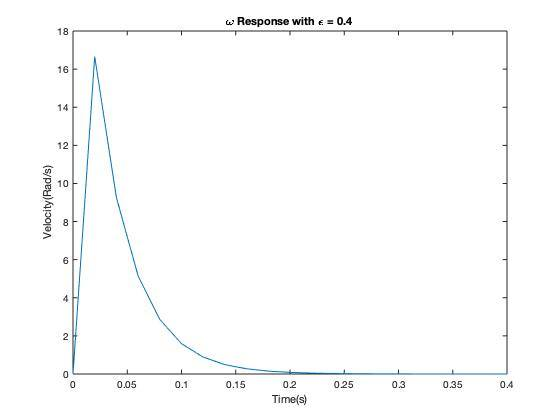
\includegraphics[width=0.8\textwidth]{./figures/lab6_omegaresponse_e_04.jpg}
	\caption{A graph of the omega response with $\epsilon = 0.4$.}
	\label{fig:}
\end{figure}

\begin{figure}[H]
	\centering
	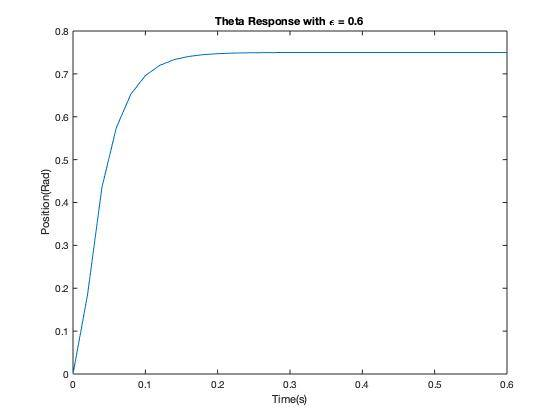
\includegraphics[width=0.8\textwidth]{./figures/lab6_thetaresponse_e_06.jpg}
	\caption{A graph of the theta response with $\epsilon = 0.6$.}
	\label{fig:}
\end{figure}

\begin{figure}[H]
	\centering
	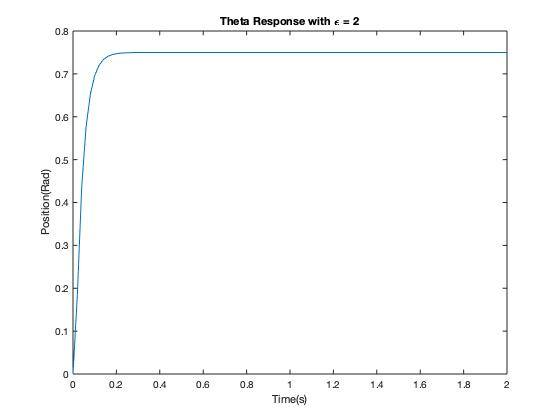
\includegraphics[width=0.8\textwidth]{./figures/lab6_thetaresponse_e_2.jpg}
	\caption{A graph of the theta response with $\epsilon = 2$.}
	\label{fig:}
\end{figure}

\begin{figure}[H]
	\centering
	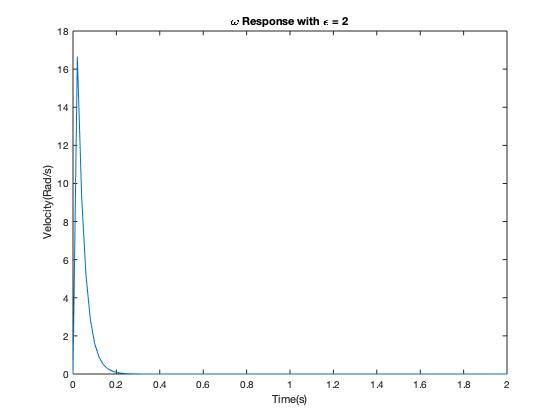
\includegraphics[width=0.8\textwidth]{./figures/lab6_omegaresponse_e_2.jpg}
	\caption{A graph of the omega response with $\epsilon = 2$.}
	\label{fig:}
\end{figure}


\section{Step 11}

\begin{figure}[H]
	\centering
 	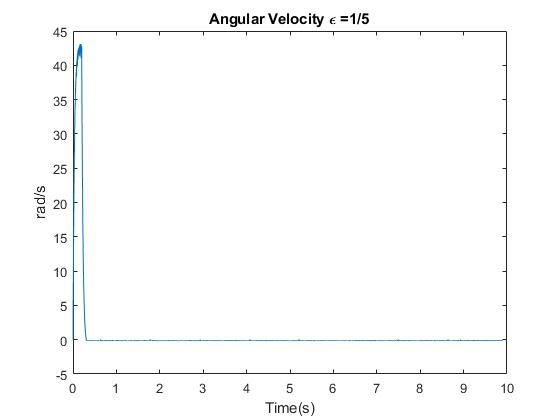
\includegraphics[width=0.8\textwidth]{./figures/lab6_angularvelocitye5.jpg}
	\caption{A graph of the angular velocity with $\epsilon = \frac{1}{5}$.}
	\label{fig:}
\end{figure}

\section{Step 12}
\begin{figure}[H]
	\centering
	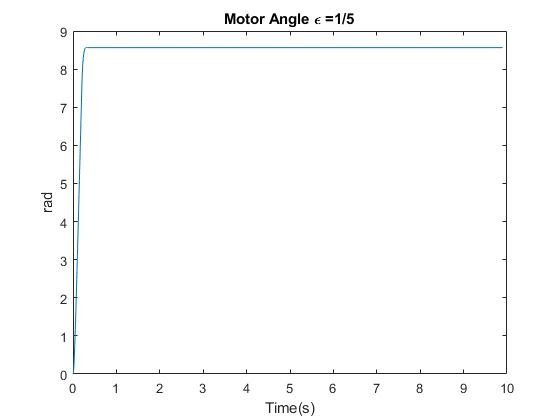
\includegraphics[width=0.8\textwidth]{./figures/lab6_motorangle_e_5.jpg}
	\caption{A graph of the motor angle with $\epsilon = \frac{1}{5}$.}
	\label{fig:}
\end{figure}

\begin{figure}[H]
	\centering
	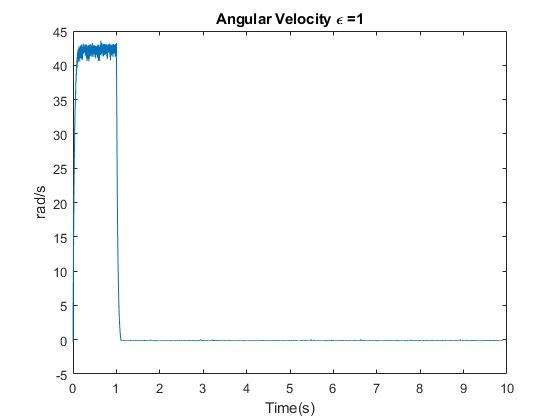
\includegraphics[width=0.8\textwidth]{./figures/lab6_angularvelocitye1.jpg}
	\caption{A graph of the angular velocity with $\epsilon = 5$.}
	\label{fig:}
\end{figure}

\section{Step 13}
\begin{figure}[H]
	\centering
 	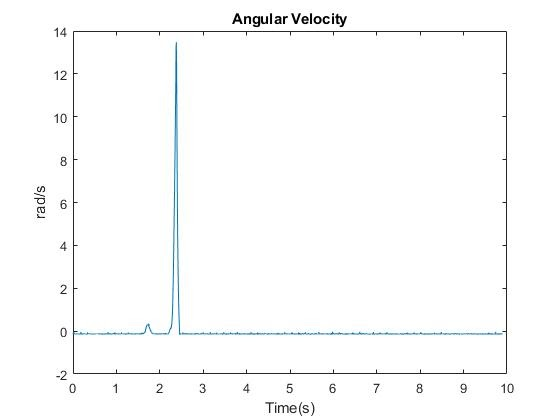
\includegraphics[width=0.8\textwidth]{./figures/lab6_angularvelocity_manual.jpg}
	\caption{A graph of the angular velocity with manual input.}
	\label{fig:}
\end{figure}

\begin{figure}[H]
	\centering
	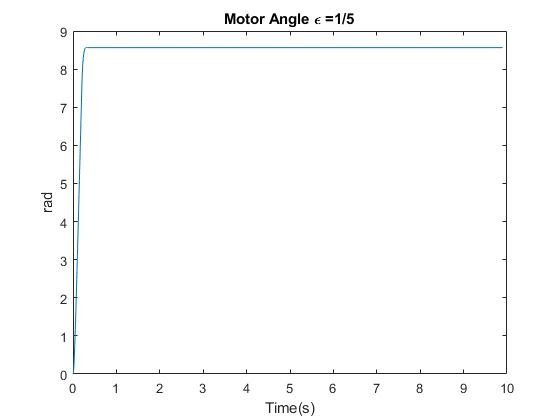
\includegraphics[width=0.8\textwidth]{./figures/lab6_motorangle_e_5.jpg}
	\caption{A graph of the motor angle with manual input.}
	\label{fig:}
\end{figure}

\section{Comments}

The shape of the Motor Angle plot with$\epsilon = 1$ and the shape of the Motor  Angle plot of simulation impulse response are roughly similar, they both have the tendency that the motor angle go up with time and keep stable when reach the stability. But the value for the stability are different among them(44 \& 1.02), and the slope of the plot before reaching the stability are different  as well, the motor angle with $\epsilon = 1$ is smaller than the impulse response.  And there is no delay on motor angle with $\epsilon = 1$, which means the reaction starting right from time 0, but there is roughly 2.3 seconds delay on the impulse response(angular velocity).

The shape of the Motor Angle plot with $\epsilon = 1/5$ and the shape of the Motor  Angle plot of simulation impulse response are roughly similar, they both have the tendency that the motor angle go up with time and keep stable when reach the stability. But the value for the stability are different among them(8.5 \& 1.02), and the slope of the plot before reaching the stability are different  as well, the motor angle with $\epsilon = 1/5$  is smaller than the impulse response.  And there is no delay on motor angle with $\epsilon = 1/5 $, which means the reaction starting right from time 0, but there is roughly 2.3 seconds delay on the impulse response(angular velocity).

The shape of the Motor Angular velocity  plot with $\epsilon = 1$ and the shape of the Motor  Angular velocity plot of simulation impulse both go down to zero after reaching the highest point.. But the value for the highest point are different among them(43 \& 13.5). There is an about 2 second delay on impulse response angular velocity, and  as the angular velocity for impulse response reaching the highest point, it immediately goes down, with no time remaining the highest angular velocity. But for the Motor Angular velocity with $\epsilon = 1$, there is no time delay, which  means, starts form time 0. And as the Motor Angular velocity with $\epsilon = 1$ reaching the highest point, it remains about 1 second then goes down to zero.

The shape of the Motor Angular velocity  plot with $\epsilon = 1/5$ and the shape of the Motor Angular velocity plot of simulation impulse are roughly the same. But the value for the highest point are different among them(43 \& 13.5). There is an about 2 second delay on impulse response angular velocity, but there is no time delay on the plot with $\epsilon = 1/5$.

